\documentclass{article}

\usepackage{fullpage}
\usepackage[brazilian]{babel}
\usepackage[utf8]{inputenc}
\usepackage[T1]{fontenc}

\usepackage[a5paper]{geometry}
\renewcommand{\familydefault}{\sfdefault}
\usepackage[scaled=1]{helvet}
\usepackage[helvet]{sfmath}
\everymath={\sf}
\usepackage{pdflscape}
\usepackage{rotating}

\usepackage{tikz}
\usetikzlibrary{calc}

\usepackage{graphicx}
\graphicspath{{./images/}}

\usepackage{parskip}
\usepackage[colorinlistoftodos]{todonotes}
\usepackage[colorlinks=true, allcolors=blue]{hyperref}

\title{Manual Do Calouro}
\author{CALICO - Centro Acadêmico Livre da Computação}
\setcounter{tocdepth}{2}

\begin{document}


% Capa
\newgeometry{margin=0em,top=0em}
    \vspace{5cm}
    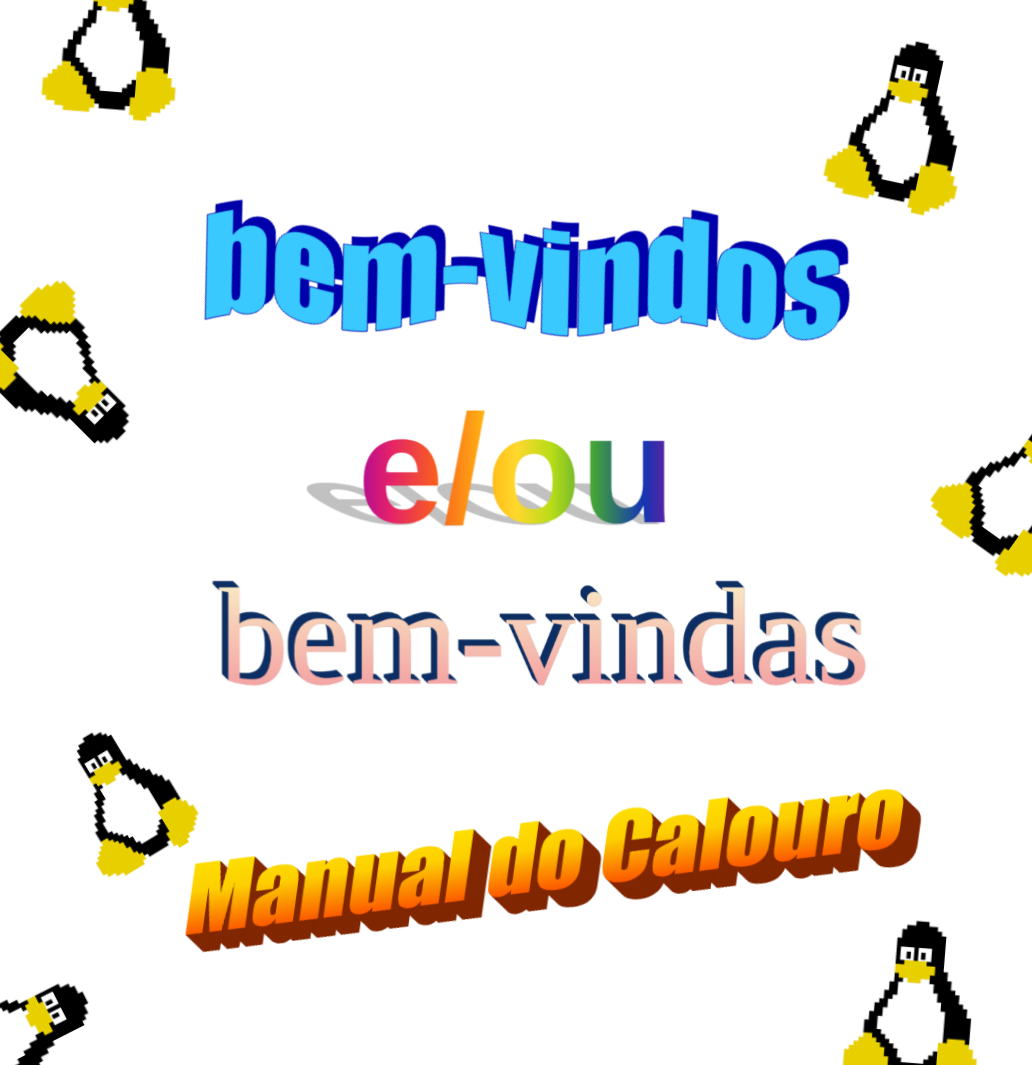
\includegraphics[width=\paperwidth,height=\paperheight]{capa}
\restoregeometry
% /Capa

\newpage
\thispagestyle{empty} % No header/footer on the blank page
\mbox{} % Adds an empty box, effectively creating a blank page
\newpage

\newpage
\thispagestyle{empty} % No header/footer on the blank page
\mbox{} % Adds an empty box, effectively creating a blank page
\newpage

\maketitle
\tableofcontents

\clearpage


\section{Ferramentas e assistências}
\subsection{Apoio Psicológico}
\subsubsection{SAPSI}
O Serviço de Atenção Psicológica é uma clínica-escola, onde os alunos estagiários do curso de Psicologia prestam um serviço de Acolhimento.
%O acolhimento psicológico é um tipo de intervenção psicológica que acolhe a pessoa no exato momento de sua urgência, não precisando de agendamento prévio.
Portanto, em casos de urgência, você pode comparecer ao Departamento de Psicologia, no Centro de Filosofia e Ciências Humanas, bloco D, 2º andar.
Não se sinta mal em pedir ajuda, sua saúde mental vem em primeiro lugar.

Horário de Funcionamento:

Segunda a sexta-feira: das 8h às 20h

\subsection{CAGR e Moodle}

O Sistema de Controle Acadêmico da Graduação, CAGR, é a principal ferramenta para acompanhar seu desempenho no curso. Lá, você tem acesso ao fórum da graduação, grade de horários, atestado de matrícula, entre outras coisas (os mais curiosos vão ter vastos dados da universidade para encontrar). Para se cadastrar, entre em cagr.ufsc.br e clique em “primeiro acesso”.

O Moodle contém as turmas em que você está matriculado (podendo alguma não estar, se o tópico não foi aberto), sendo possível então o professor de cada disciplina disponibilizar slides, fazer um controle de notas ou faltas, ou até mesmo aplicar provas por essa plataforma. É onde, geralmente, seu professor coloca o seu material de estudo e passa recados importantes. Como o acesso é unificado, basta entrar em moodle.ufsc.br e entrar com o que você previamente se cadastrou no CAGR. Nada como um sentimento de “notas da prova no moodle” (desespero).

\subsection{Acesso a Internet} 
Para acessar a rede “eduroam”, é necessário ter um cadastro no \href{idufsc.ufsc.br}{idufsc.ufsc.br}. Entre no site e clique em “Criar Usuário” digitando seu CPF e data de nascimento. Você receberá um e-mail com uma confirmação e um link para você criar seu usuário e senha. Depois, siga esses passos ao conectar: 
\begin{enumerate}
\item Modo de Segurança: WPA2-Enterprise (Wi-Fi Protected Access II – Enterprise)

\item Método EAP: TTLS (Tunneled Transport Layer Security)

\item Autenticação da Fase 2: PAP (Password Authentication Protocol)

\item Domínio: ufsc.br

\item Identidade: seu.idufsc@ufsc.br (aqui você também pode colocar sua matrícula)
Senha: sua.senha
\end{enumerate}


    \subsection{Vivendo em Florianópolis}
    \subsubsection{Ônibus}
Em Florianópolis, o único meio de transporte público disponível é o ônibus. As linhas são todas baseadas em terminais integrados espalhados pela cidade, sendo os mais próximos da UFSC o TITRI (Terminal de Integração da Trindade) e o TICEN (Terminal de Integração do Centro), desse jeito, se você pega um ônibus e desce em um terminal, pode entrar em outro ônibus e não pagar nada! Caso você possua qualquer um dos cartões da empresa, é possível integrar (lê-se, passar a catraca do ônibus sem pagar) em qualquer ponto da cidade, bastando utilizar o mesmo cartão dentro de um período estipulado (atualmente esse período é de aproximadamente 3h).

Além disso, os ônibus saem de seus respectivos lugares em horários específicos, e são, geralmente, bem pontuais.
Portanto, antes de sair de casa, verifique os horários do seu ônibus \href{consorciofenix.com.br}{consorciofenix .com.br}.
Ou baixe o app \href{https://play.google.com/store/search?q=floripa%20no%20ponto}{Floripa no Ponto 2.0}, esse app é péssimo para pesquisar qual ônibus pegar do ponto A ao ponto B, mas fornece a localização em tempo real de quase todos ônibus. Isso lhe poupará uma boa espera. Há também apps variados de consulta de horários disponíveis para serem baixados (o Google Maps é bem prático).

\subsubsection{Cartão de Estudante}

Você também pode fazer o seu cartão de estudante e pegar apenas meia tarifa.
Para isso, você precisará ir ao SETUF, localizado no TICEN, levando os documentos necessários que estão listados em \href{https://www.setuf.com.br/facil/perguntas-frequentes/perguntas-estudante/}{https://www.setuf.com.br/facil/perguntas-frequentes/perguntas-estudante/}.

O comprovante de matrícula disponível no seu \href{https://cagr.sistemas.ufsc.br/relatorios/aluno/atestadoMatricula?download}{CAGR},
que é assinado digitalmente como é possível de se verificar no rodapé, constando como "regularmente matriculado" deveria ser suficiente para comprovar seu vínculo acadêmico.
Porém é comum haver atrito para ser aceito, nesses casos procure auxílio do movimento estudantil (CALICO e DCE) ou da coordenação do curso (cco@contato. ufsc.br).

É altamente recomendável que se faça o cartão.
Para recadastros e recargas do cartão, é possível fazer tanto em qualquer um dos terminais integrados quanto inteiramente no aplicativo \href{https://play.google.com/store/apps/details?id=br.com.henkoti.empresa1.smpay}{SI.GO}

%    \input{content/tools/student_card}
    \subsection{Classificados da UFSC}
Se você ainda está a procura de casas, móveis, gatos, cachorros, bicicletas, microondas ou plantas, entre no site \url{classificados.inf.ufsc.br}
ou nos grupos públicos de facebook para achar o que você precisa. Se você não mora perto da universidade, também pode pesquisar "Classificados e o nome do seu bairro"  para achar o seu respectivo grupo.


% \subsection{O que está acontecendo com a UFSC e outras universidades?}
% No primeiro semestre deste ano, o Ministério da Educação anunciou um bloqueio de cerca de 30\% do orçamento de três universidades federais: UFBA, UnB e UFF. O ministro afirmou que "universidades que, em vez de procurar melhorar o desempenho acadêmico, estiverem fazendo balbúrdia, terão verbas reduzidas. A universidade deve estar com sobra de dinheiro para fazer bagunça e evento ridículo", disse ele a respeito de eventos realizados nestas universidades:
% \begin{itemize}
% \item na UFBA, o 15º CONEB (Conselho de Entidades de Base) e a 11ª Bienal da UNE (União Nacional dos Estudantes);
% \item na UFF, o 6º ENUNE (Encontro de Estudantes Negros, Negras e Cotistas da UNE);
% \item na UnB, o III ENE (Encontro Nacional da Educação) e o 57º CONUNE (Congresso da UNE).
% \end{itemize}
% Ficou claro para todos que a medida tinha motivações ideológicas e, após repercussões, o ministério decidiu expandir o bloqueio a todas as universidades e institutos federais.
% 
% Em resposta a isso, estudantes de todo o país se mobilizaram para a construção de um grande ato em defesa da educação. 52 centros acadêmicos da UFSC, incluido o CALICO (em assembleia dos estudantes de Ciência da Computação), decidiram se posicionar contra esses ataques, compondo a grande manifestação do dia 15 de Maio. Nesse mesmo dia, o presidente Jair Bolsonaro, do hotel que estava hospedado em Dallas (Texas), chamou os estudantes de “idiotas úteis” e assinou um decreto que retira dos reitores a autonomia de nomear e designar cargos de gestão nas universidades federais, como pró-reitores (que são como ministros da universidade), diretores de centros, entre outros.
% 
% O bloqueio permanece e os ataques à educação continuam, dessa vez caracterizados por um amplo projeto que ameaça o caráter público e social das universidades, chamado Programa Institutos e Universidades Empreendedoras e Inovadoras, ou Future-se. É nosso dever como estudantes lutar pelo desenvolvimento técnico-científico e pela produção artístico-cultural, realizados no ensino superior público. Já foi declarado que a UFSC pode não conseguir se manter nesse segundo semestre, e, com isso, o CALICO pretende fazer eventos informativos e de contextualização para que todos possam entender e fazer parte da defesa da Universidade. 
% 

\section{Ferramentas e assistências}
\subsection{Apoio Psicológico}
\subsubsection{SAPSI}
O Serviço de Atenção Psicológica é uma clínica-escola, onde os alunos estagiários do curso de Psicologia prestam um serviço de Acolhimento.
%O acolhimento psicológico é um tipo de intervenção psicológica que acolhe a pessoa no exato momento de sua urgência, não precisando de agendamento prévio.
Portanto, em casos de urgência, você pode comparecer ao Departamento de Psicologia, no Centro de Filosofia e Ciências Humanas, bloco D, 2º andar.
Não se sinta mal em pedir ajuda, sua saúde mental vem em primeiro lugar.

Horário de Funcionamento:

Segunda a sexta-feira: das 8h às 20h

\subsection{CAGR e Moodle}

O Sistema de Controle Acadêmico da Graduação, CAGR, é a principal ferramenta para acompanhar seu desempenho no curso. Lá, você tem acesso ao fórum da graduação, grade de horários, atestado de matrícula, entre outras coisas (os mais curiosos vão ter vastos dados da universidade para encontrar). Para se cadastrar, entre em cagr.ufsc.br e clique em “primeiro acesso”.

O Moodle contém as turmas em que você está matriculado (podendo alguma não estar, se o tópico não foi aberto), sendo possível então o professor de cada disciplina disponibilizar slides, fazer um controle de notas ou faltas, ou até mesmo aplicar provas por essa plataforma. É onde, geralmente, seu professor coloca o seu material de estudo e passa recados importantes. Como o acesso é unificado, basta entrar em moodle.ufsc.br e entrar com o que você previamente se cadastrou no CAGR. Nada como um sentimento de “notas da prova no moodle” (desespero).

\subsection{Acesso a Internet} 
Para acessar a rede “eduroam”, é necessário ter um cadastro no \href{idufsc.ufsc.br}{idufsc.ufsc.br}. Entre no site e clique em “Criar Usuário” digitando seu CPF e data de nascimento. Você receberá um e-mail com uma confirmação e um link para você criar seu usuário e senha. Depois, siga esses passos ao conectar: 
\begin{enumerate}
\item Modo de Segurança: WPA2-Enterprise (Wi-Fi Protected Access II – Enterprise)

\item Método EAP: TTLS (Tunneled Transport Layer Security)

\item Autenticação da Fase 2: PAP (Password Authentication Protocol)

\item Domínio: ufsc.br

\item Identidade: seu.idufsc@ufsc.br (aqui você também pode colocar sua matrícula)
Senha: sua.senha
\end{enumerate}


    \subsection{Vivendo em Florianópolis}
    \subsubsection{Ônibus}
Em Florianópolis, o único meio de transporte público disponível é o ônibus. As linhas são todas baseadas em terminais integrados espalhados pela cidade, sendo os mais próximos da UFSC o TITRI (Terminal de Integração da Trindade) e o TICEN (Terminal de Integração do Centro), desse jeito, se você pega um ônibus e desce em um terminal, pode entrar em outro ônibus e não pagar nada! Caso você possua qualquer um dos cartões da empresa, é possível integrar (lê-se, passar a catraca do ônibus sem pagar) em qualquer ponto da cidade, bastando utilizar o mesmo cartão dentro de um período estipulado (atualmente esse período é de aproximadamente 3h).

Além disso, os ônibus saem de seus respectivos lugares em horários específicos, e são, geralmente, bem pontuais.
Portanto, antes de sair de casa, verifique os horários do seu ônibus \href{consorciofenix.com.br}{consorciofenix .com.br}.
Ou baixe o app \href{https://play.google.com/store/search?q=floripa%20no%20ponto}{Floripa no Ponto 2.0}, esse app é péssimo para pesquisar qual ônibus pegar do ponto A ao ponto B, mas fornece a localização em tempo real de quase todos ônibus. Isso lhe poupará uma boa espera. Há também apps variados de consulta de horários disponíveis para serem baixados (o Google Maps é bem prático).

\subsubsection{Cartão de Estudante}

Você também pode fazer o seu cartão de estudante e pegar apenas meia tarifa.
Para isso, você precisará ir ao SETUF, localizado no TICEN, levando os documentos necessários que estão listados em \href{https://www.setuf.com.br/facil/perguntas-frequentes/perguntas-estudante/}{https://www.setuf.com.br/facil/perguntas-frequentes/perguntas-estudante/}.

O comprovante de matrícula disponível no seu \href{https://cagr.sistemas.ufsc.br/relatorios/aluno/atestadoMatricula?download}{CAGR},
que é assinado digitalmente como é possível de se verificar no rodapé, constando como "regularmente matriculado" deveria ser suficiente para comprovar seu vínculo acadêmico.
Porém é comum haver atrito para ser aceito, nesses casos procure auxílio do movimento estudantil (CALICO e DCE) ou da coordenação do curso (cco@contato. ufsc.br).

É altamente recomendável que se faça o cartão.
Para recadastros e recargas do cartão, é possível fazer tanto em qualquer um dos terminais integrados quanto inteiramente no aplicativo \href{https://play.google.com/store/apps/details?id=br.com.henkoti.empresa1.smpay}{SI.GO}

%    \input{content/tools/student_card}
    \subsection{Classificados da UFSC}
Se você ainda está a procura de casas, móveis, gatos, cachorros, bicicletas, microondas ou plantas, entre no site \url{classificados.inf.ufsc.br}
ou nos grupos públicos de facebook para achar o que você precisa. Se você não mora perto da universidade, também pode pesquisar "Classificados e o nome do seu bairro"  para achar o seu respectivo grupo.


% \subsection{O que está acontecendo com a UFSC e outras universidades?}
% No primeiro semestre deste ano, o Ministério da Educação anunciou um bloqueio de cerca de 30\% do orçamento de três universidades federais: UFBA, UnB e UFF. O ministro afirmou que "universidades que, em vez de procurar melhorar o desempenho acadêmico, estiverem fazendo balbúrdia, terão verbas reduzidas. A universidade deve estar com sobra de dinheiro para fazer bagunça e evento ridículo", disse ele a respeito de eventos realizados nestas universidades:
% \begin{itemize}
% \item na UFBA, o 15º CONEB (Conselho de Entidades de Base) e a 11ª Bienal da UNE (União Nacional dos Estudantes);
% \item na UFF, o 6º ENUNE (Encontro de Estudantes Negros, Negras e Cotistas da UNE);
% \item na UnB, o III ENE (Encontro Nacional da Educação) e o 57º CONUNE (Congresso da UNE).
% \end{itemize}
% Ficou claro para todos que a medida tinha motivações ideológicas e, após repercussões, o ministério decidiu expandir o bloqueio a todas as universidades e institutos federais.
% 
% Em resposta a isso, estudantes de todo o país se mobilizaram para a construção de um grande ato em defesa da educação. 52 centros acadêmicos da UFSC, incluido o CALICO (em assembleia dos estudantes de Ciência da Computação), decidiram se posicionar contra esses ataques, compondo a grande manifestação do dia 15 de Maio. Nesse mesmo dia, o presidente Jair Bolsonaro, do hotel que estava hospedado em Dallas (Texas), chamou os estudantes de “idiotas úteis” e assinou um decreto que retira dos reitores a autonomia de nomear e designar cargos de gestão nas universidades federais, como pró-reitores (que são como ministros da universidade), diretores de centros, entre outros.
% 
% O bloqueio permanece e os ataques à educação continuam, dessa vez caracterizados por um amplo projeto que ameaça o caráter público e social das universidades, chamado Programa Institutos e Universidades Empreendedoras e Inovadoras, ou Future-se. É nosso dever como estudantes lutar pelo desenvolvimento técnico-científico e pela produção artístico-cultural, realizados no ensino superior público. Já foi declarado que a UFSC pode não conseguir se manter nesse segundo semestre, e, com isso, o CALICO pretende fazer eventos informativos e de contextualização para que todos possam entender e fazer parte da defesa da Universidade. 
% 

\section{Ferramentas e assistências}
\subsection{Apoio Psicológico}
\subsubsection{SAPSI}
O Serviço de Atenção Psicológica é uma clínica-escola, onde os alunos estagiários do curso de Psicologia prestam um serviço de Acolhimento.
%O acolhimento psicológico é um tipo de intervenção psicológica que acolhe a pessoa no exato momento de sua urgência, não precisando de agendamento prévio.
Portanto, em casos de urgência, você pode comparecer ao Departamento de Psicologia, no Centro de Filosofia e Ciências Humanas, bloco D, 2º andar.
Não se sinta mal em pedir ajuda, sua saúde mental vem em primeiro lugar.

Horário de Funcionamento:

Segunda a sexta-feira: das 8h às 20h

\subsection{CAGR e Moodle}

O Sistema de Controle Acadêmico da Graduação, CAGR, é a principal ferramenta para acompanhar seu desempenho no curso. Lá, você tem acesso ao fórum da graduação, grade de horários, atestado de matrícula, entre outras coisas (os mais curiosos vão ter vastos dados da universidade para encontrar). Para se cadastrar, entre em cagr.ufsc.br e clique em “primeiro acesso”.

O Moodle contém as turmas em que você está matriculado (podendo alguma não estar, se o tópico não foi aberto), sendo possível então o professor de cada disciplina disponibilizar slides, fazer um controle de notas ou faltas, ou até mesmo aplicar provas por essa plataforma. É onde, geralmente, seu professor coloca o seu material de estudo e passa recados importantes. Como o acesso é unificado, basta entrar em moodle.ufsc.br e entrar com o que você previamente se cadastrou no CAGR. Nada como um sentimento de “notas da prova no moodle” (desespero).

\subsection{Acesso a Internet} 
Para acessar a rede “eduroam”, é necessário ter um cadastro no \href{idufsc.ufsc.br}{idufsc.ufsc.br}. Entre no site e clique em “Criar Usuário” digitando seu CPF e data de nascimento. Você receberá um e-mail com uma confirmação e um link para você criar seu usuário e senha. Depois, siga esses passos ao conectar: 
\begin{enumerate}
\item Modo de Segurança: WPA2-Enterprise (Wi-Fi Protected Access II – Enterprise)

\item Método EAP: TTLS (Tunneled Transport Layer Security)

\item Autenticação da Fase 2: PAP (Password Authentication Protocol)

\item Domínio: ufsc.br

\item Identidade: seu.idufsc@ufsc.br (aqui você também pode colocar sua matrícula)
Senha: sua.senha
\end{enumerate}


    \subsection{Vivendo em Florianópolis}
    \subsubsection{Ônibus}
Em Florianópolis, o único meio de transporte público disponível é o ônibus. As linhas são todas baseadas em terminais integrados espalhados pela cidade, sendo os mais próximos da UFSC o TITRI (Terminal de Integração da Trindade) e o TICEN (Terminal de Integração do Centro), desse jeito, se você pega um ônibus e desce em um terminal, pode entrar em outro ônibus e não pagar nada! Caso você possua qualquer um dos cartões da empresa, é possível integrar (lê-se, passar a catraca do ônibus sem pagar) em qualquer ponto da cidade, bastando utilizar o mesmo cartão dentro de um período estipulado (atualmente esse período é de aproximadamente 3h).

Além disso, os ônibus saem de seus respectivos lugares em horários específicos, e são, geralmente, bem pontuais.
Portanto, antes de sair de casa, verifique os horários do seu ônibus \href{consorciofenix.com.br}{consorciofenix .com.br}.
Ou baixe o app \href{https://play.google.com/store/search?q=floripa%20no%20ponto}{Floripa no Ponto 2.0}, esse app é péssimo para pesquisar qual ônibus pegar do ponto A ao ponto B, mas fornece a localização em tempo real de quase todos ônibus. Isso lhe poupará uma boa espera. Há também apps variados de consulta de horários disponíveis para serem baixados (o Google Maps é bem prático).

\subsubsection{Cartão de Estudante}

Você também pode fazer o seu cartão de estudante e pegar apenas meia tarifa.
Para isso, você precisará ir ao SETUF, localizado no TICEN, levando os documentos necessários que estão listados em \href{https://www.setuf.com.br/facil/perguntas-frequentes/perguntas-estudante/}{https://www.setuf.com.br/facil/perguntas-frequentes/perguntas-estudante/}.

O comprovante de matrícula disponível no seu \href{https://cagr.sistemas.ufsc.br/relatorios/aluno/atestadoMatricula?download}{CAGR},
que é assinado digitalmente como é possível de se verificar no rodapé, constando como "regularmente matriculado" deveria ser suficiente para comprovar seu vínculo acadêmico.
Porém é comum haver atrito para ser aceito, nesses casos procure auxílio do movimento estudantil (CALICO e DCE) ou da coordenação do curso (cco@contato. ufsc.br).

É altamente recomendável que se faça o cartão.
Para recadastros e recargas do cartão, é possível fazer tanto em qualquer um dos terminais integrados quanto inteiramente no aplicativo \href{https://play.google.com/store/apps/details?id=br.com.henkoti.empresa1.smpay}{SI.GO}

%    \input{content/tools/student_card}
    \subsection{Classificados da UFSC}
Se você ainda está a procura de casas, móveis, gatos, cachorros, bicicletas, microondas ou plantas, entre no site \url{classificados.inf.ufsc.br}
ou nos grupos públicos de facebook para achar o que você precisa. Se você não mora perto da universidade, também pode pesquisar "Classificados e o nome do seu bairro"  para achar o seu respectivo grupo.


% \subsection{O que está acontecendo com a UFSC e outras universidades?}
% No primeiro semestre deste ano, o Ministério da Educação anunciou um bloqueio de cerca de 30\% do orçamento de três universidades federais: UFBA, UnB e UFF. O ministro afirmou que "universidades que, em vez de procurar melhorar o desempenho acadêmico, estiverem fazendo balbúrdia, terão verbas reduzidas. A universidade deve estar com sobra de dinheiro para fazer bagunça e evento ridículo", disse ele a respeito de eventos realizados nestas universidades:
% \begin{itemize}
% \item na UFBA, o 15º CONEB (Conselho de Entidades de Base) e a 11ª Bienal da UNE (União Nacional dos Estudantes);
% \item na UFF, o 6º ENUNE (Encontro de Estudantes Negros, Negras e Cotistas da UNE);
% \item na UnB, o III ENE (Encontro Nacional da Educação) e o 57º CONUNE (Congresso da UNE).
% \end{itemize}
% Ficou claro para todos que a medida tinha motivações ideológicas e, após repercussões, o ministério decidiu expandir o bloqueio a todas as universidades e institutos federais.
% 
% Em resposta a isso, estudantes de todo o país se mobilizaram para a construção de um grande ato em defesa da educação. 52 centros acadêmicos da UFSC, incluido o CALICO (em assembleia dos estudantes de Ciência da Computação), decidiram se posicionar contra esses ataques, compondo a grande manifestação do dia 15 de Maio. Nesse mesmo dia, o presidente Jair Bolsonaro, do hotel que estava hospedado em Dallas (Texas), chamou os estudantes de “idiotas úteis” e assinou um decreto que retira dos reitores a autonomia de nomear e designar cargos de gestão nas universidades federais, como pró-reitores (que são como ministros da universidade), diretores de centros, entre outros.
% 
% O bloqueio permanece e os ataques à educação continuam, dessa vez caracterizados por um amplo projeto que ameaça o caráter público e social das universidades, chamado Programa Institutos e Universidades Empreendedoras e Inovadoras, ou Future-se. É nosso dever como estudantes lutar pelo desenvolvimento técnico-científico e pela produção artístico-cultural, realizados no ensino superior público. Já foi declarado que a UFSC pode não conseguir se manter nesse segundo semestre, e, com isso, o CALICO pretende fazer eventos informativos e de contextualização para que todos possam entender e fazer parte da defesa da Universidade. 
% 

\section{Ferramentas e assistências}
\subsection{Apoio Psicológico}
\subsubsection{SAPSI}
O Serviço de Atenção Psicológica é uma clínica-escola, onde os alunos estagiários do curso de Psicologia prestam um serviço de Acolhimento.
%O acolhimento psicológico é um tipo de intervenção psicológica que acolhe a pessoa no exato momento de sua urgência, não precisando de agendamento prévio.
Portanto, em casos de urgência, você pode comparecer ao Departamento de Psicologia, no Centro de Filosofia e Ciências Humanas, bloco D, 2º andar.
Não se sinta mal em pedir ajuda, sua saúde mental vem em primeiro lugar.

Horário de Funcionamento:

Segunda a sexta-feira: das 8h às 20h

\subsection{CAGR e Moodle}

O Sistema de Controle Acadêmico da Graduação, CAGR, é a principal ferramenta para acompanhar seu desempenho no curso. Lá, você tem acesso ao fórum da graduação, grade de horários, atestado de matrícula, entre outras coisas (os mais curiosos vão ter vastos dados da universidade para encontrar). Para se cadastrar, entre em cagr.ufsc.br e clique em “primeiro acesso”.

O Moodle contém as turmas em que você está matriculado (podendo alguma não estar, se o tópico não foi aberto), sendo possível então o professor de cada disciplina disponibilizar slides, fazer um controle de notas ou faltas, ou até mesmo aplicar provas por essa plataforma. É onde, geralmente, seu professor coloca o seu material de estudo e passa recados importantes. Como o acesso é unificado, basta entrar em moodle.ufsc.br e entrar com o que você previamente se cadastrou no CAGR. Nada como um sentimento de “notas da prova no moodle” (desespero).

\subsection{Acesso a Internet} 
Para acessar a rede “eduroam”, é necessário ter um cadastro no \href{idufsc.ufsc.br}{idufsc.ufsc.br}. Entre no site e clique em “Criar Usuário” digitando seu CPF e data de nascimento. Você receberá um e-mail com uma confirmação e um link para você criar seu usuário e senha. Depois, siga esses passos ao conectar: 
\begin{enumerate}
\item Modo de Segurança: WPA2-Enterprise (Wi-Fi Protected Access II – Enterprise)

\item Método EAP: TTLS (Tunneled Transport Layer Security)

\item Autenticação da Fase 2: PAP (Password Authentication Protocol)

\item Domínio: ufsc.br

\item Identidade: seu.idufsc@ufsc.br (aqui você também pode colocar sua matrícula)
Senha: sua.senha
\end{enumerate}


    \subsection{Vivendo em Florianópolis}
    \subsubsection{Ônibus}
Em Florianópolis, o único meio de transporte público disponível é o ônibus. As linhas são todas baseadas em terminais integrados espalhados pela cidade, sendo os mais próximos da UFSC o TITRI (Terminal de Integração da Trindade) e o TICEN (Terminal de Integração do Centro), desse jeito, se você pega um ônibus e desce em um terminal, pode entrar em outro ônibus e não pagar nada! Caso você possua qualquer um dos cartões da empresa, é possível integrar (lê-se, passar a catraca do ônibus sem pagar) em qualquer ponto da cidade, bastando utilizar o mesmo cartão dentro de um período estipulado (atualmente esse período é de aproximadamente 3h).

Além disso, os ônibus saem de seus respectivos lugares em horários específicos, e são, geralmente, bem pontuais.
Portanto, antes de sair de casa, verifique os horários do seu ônibus \href{consorciofenix.com.br}{consorciofenix .com.br}.
Ou baixe o app \href{https://play.google.com/store/search?q=floripa%20no%20ponto}{Floripa no Ponto 2.0}, esse app é péssimo para pesquisar qual ônibus pegar do ponto A ao ponto B, mas fornece a localização em tempo real de quase todos ônibus. Isso lhe poupará uma boa espera. Há também apps variados de consulta de horários disponíveis para serem baixados (o Google Maps é bem prático).

\subsubsection{Cartão de Estudante}

Você também pode fazer o seu cartão de estudante e pegar apenas meia tarifa.
Para isso, você precisará ir ao SETUF, localizado no TICEN, levando os documentos necessários que estão listados em \href{https://www.setuf.com.br/facil/perguntas-frequentes/perguntas-estudante/}{https://www.setuf.com.br/facil/perguntas-frequentes/perguntas-estudante/}.

O comprovante de matrícula disponível no seu \href{https://cagr.sistemas.ufsc.br/relatorios/aluno/atestadoMatricula?download}{CAGR},
que é assinado digitalmente como é possível de se verificar no rodapé, constando como "regularmente matriculado" deveria ser suficiente para comprovar seu vínculo acadêmico.
Porém é comum haver atrito para ser aceito, nesses casos procure auxílio do movimento estudantil (CALICO e DCE) ou da coordenação do curso (cco@contato. ufsc.br).

É altamente recomendável que se faça o cartão.
Para recadastros e recargas do cartão, é possível fazer tanto em qualquer um dos terminais integrados quanto inteiramente no aplicativo \href{https://play.google.com/store/apps/details?id=br.com.henkoti.empresa1.smpay}{SI.GO}

%    \input{content/tools/student_card}
    \subsection{Classificados da UFSC}
Se você ainda está a procura de casas, móveis, gatos, cachorros, bicicletas, microondas ou plantas, entre no site \url{classificados.inf.ufsc.br}
ou nos grupos públicos de facebook para achar o que você precisa. Se você não mora perto da universidade, também pode pesquisar "Classificados e o nome do seu bairro"  para achar o seu respectivo grupo.


% \subsection{O que está acontecendo com a UFSC e outras universidades?}
% No primeiro semestre deste ano, o Ministério da Educação anunciou um bloqueio de cerca de 30\% do orçamento de três universidades federais: UFBA, UnB e UFF. O ministro afirmou que "universidades que, em vez de procurar melhorar o desempenho acadêmico, estiverem fazendo balbúrdia, terão verbas reduzidas. A universidade deve estar com sobra de dinheiro para fazer bagunça e evento ridículo", disse ele a respeito de eventos realizados nestas universidades:
% \begin{itemize}
% \item na UFBA, o 15º CONEB (Conselho de Entidades de Base) e a 11ª Bienal da UNE (União Nacional dos Estudantes);
% \item na UFF, o 6º ENUNE (Encontro de Estudantes Negros, Negras e Cotistas da UNE);
% \item na UnB, o III ENE (Encontro Nacional da Educação) e o 57º CONUNE (Congresso da UNE).
% \end{itemize}
% Ficou claro para todos que a medida tinha motivações ideológicas e, após repercussões, o ministério decidiu expandir o bloqueio a todas as universidades e institutos federais.
% 
% Em resposta a isso, estudantes de todo o país se mobilizaram para a construção de um grande ato em defesa da educação. 52 centros acadêmicos da UFSC, incluido o CALICO (em assembleia dos estudantes de Ciência da Computação), decidiram se posicionar contra esses ataques, compondo a grande manifestação do dia 15 de Maio. Nesse mesmo dia, o presidente Jair Bolsonaro, do hotel que estava hospedado em Dallas (Texas), chamou os estudantes de “idiotas úteis” e assinou um decreto que retira dos reitores a autonomia de nomear e designar cargos de gestão nas universidades federais, como pró-reitores (que são como ministros da universidade), diretores de centros, entre outros.
% 
% O bloqueio permanece e os ataques à educação continuam, dessa vez caracterizados por um amplo projeto que ameaça o caráter público e social das universidades, chamado Programa Institutos e Universidades Empreendedoras e Inovadoras, ou Future-se. É nosso dever como estudantes lutar pelo desenvolvimento técnico-científico e pela produção artístico-cultural, realizados no ensino superior público. Já foi declarado que a UFSC pode não conseguir se manter nesse segundo semestre, e, com isso, o CALICO pretende fazer eventos informativos e de contextualização para que todos possam entender e fazer parte da defesa da Universidade. 
% 


\newgeometry{margin=0pt}
\begin{figure}[p]
    \centering
    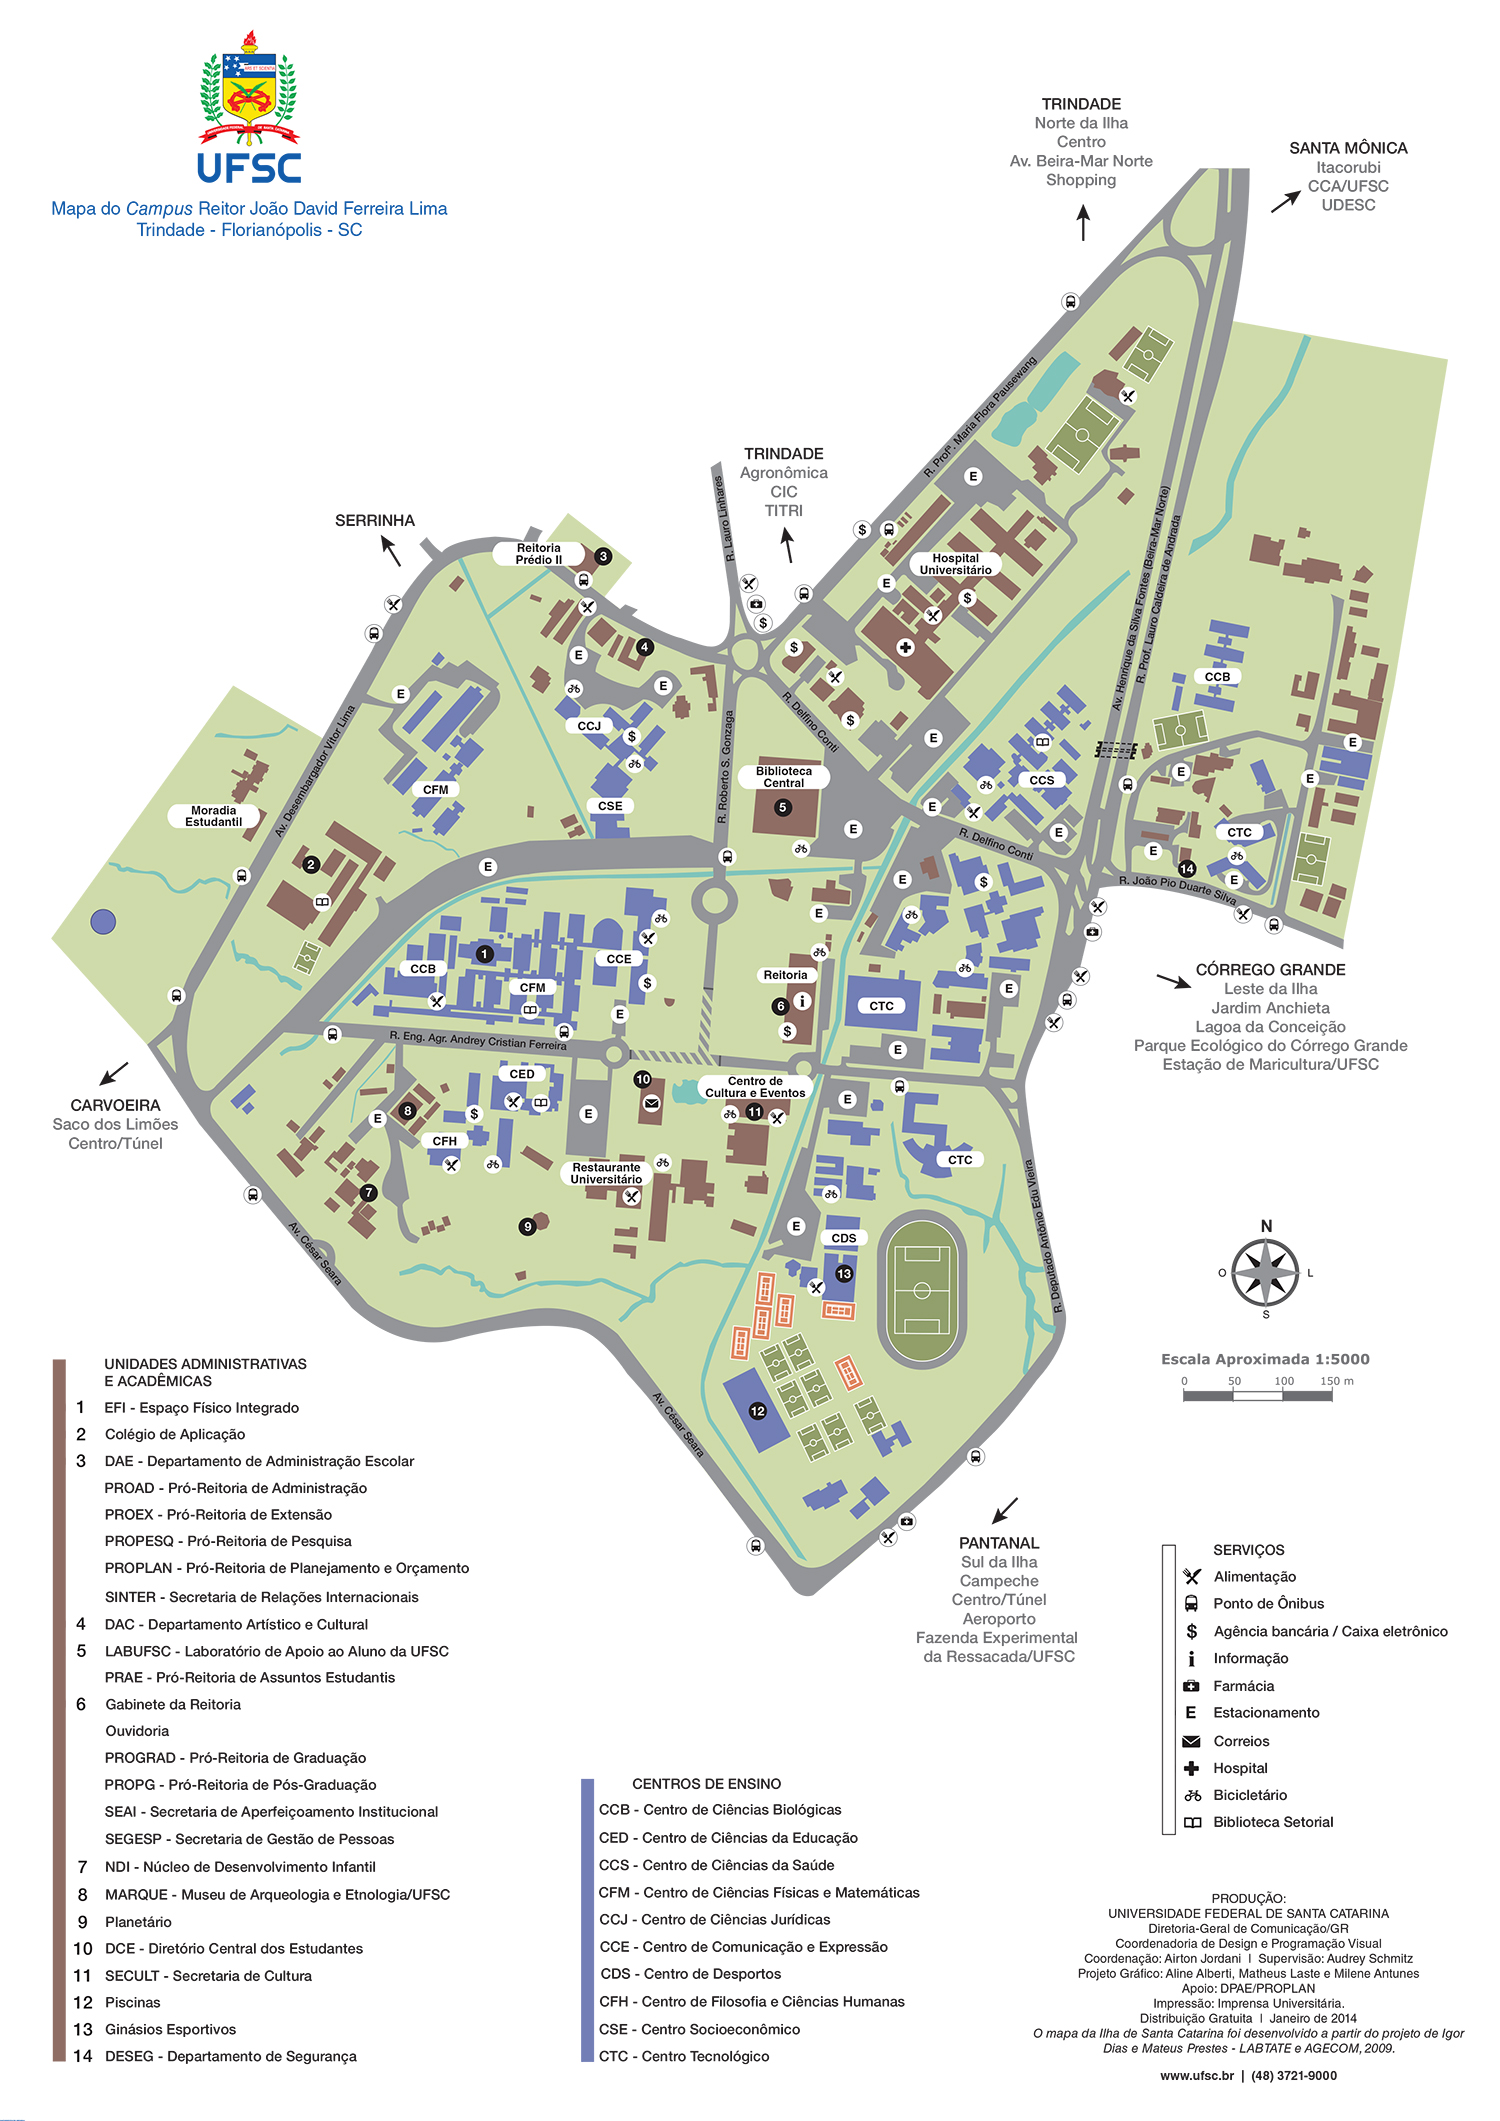
\includegraphics[width=\paperwidth, height=\paperheight]{mapa_UFSC_2014_1500x2121}
\end{figure}
\restoregeometry

\newpage
\thispagestyle{empty} % No header/footer on the blank page
\mbox{} % Adds an empty box, effectively creating a blank page
\newpage

\clearpage


% Contra-Capa
\thispagestyle{empty}
\begin{tikzpicture}[thick,scale=0.05,every node/.style={scale=0.26},overlay]
  \node[anchor=north east,inner sep=0pt] at ($(current page.south west)+(90cm,-277cm)$) {
     \includegraphics{CALICO}
  };
  
\end{tikzpicture}

\begin{tikzpicture}[thick,scale=0.05,every node/.style={scale=0.12},overlay]
    \node[anchor=north west,inner sep=0pt] at ($(current page.south west)+(130cm,-233cm)$) {
     
\includegraphics{p2p}
  };
  
\end{tikzpicture}
% /Contra-Capa

\end{document}
